\documentclass[11pt]{article}
\usepackage[utf8]{inputenc}
\usepackage[lmargin=2cm, tmargin=3cm, rmargin=2cm, bmargin=2cm, headheight=5cm]{geometry}
\usepackage{graphicx}
\usepackage{subfigure}
\usepackage{enumerate}
\usepackage{listings}
\usepackage{caption}
\usepackage{float}
\usepackage[hidelinks]{hyperref}
\usepackage{fancyhdr}
\usepackage{amsmath}
\usepackage{needspace}

\pagestyle{fancy}{
\rhead{\includegraphics[width=30mm]{../other/logo_ist.png}}
\lhead{TCFE lab report}
}


\begin{document}
\thispagestyle{empty}
\begin{figure}[h]
	\centering
	\includegraphics[width=.6\textwidth]{../../figlib/IST_A_CMYK_POS.pdf}
\end{figure}

\begin{center}
	\huge{Circuit Theory and Electronic Fundamentals}
	
	\huge{Lab Report - T3}
	
	\vspace{30pt}
	
	\large{Professor: José Sousa}
	
	\vspace{20pt}
	
	\large{95801 - João Domingos}
	
	\large{96382 - Francisco Cadavez}
	
	\large{97087 - Miguel Fernandes}
	
	\vspace{20pt}
	
	\large{April $26^{th}$ 2021}
\end{center}

\pagebreak
\tableofcontents

\pagebreak
\section{Introduction}
\hspace{12pt} In this laboratorial session we were tasked to create an AC/DC converter circuit (whose basic layout is described in Figure \ref{fig:ac_dc}), this includes a transformer, a full-wave rectifier an envelope detector and a voltage regulator circuits. The specific arquitecture for these sub-circuits is described in Figure \ref{fig:circuit}.

\begin{figure}[h]
	\centering
	\includegraphics[width=.5\textwidth, trim={0 4cm 0 4cm}, clip]{AC_DC.pdf}
	\caption{AC/DC converter circuit layout}
	\label{fig:ac_dc}
\end{figure}
 
 \begin{figure}[h]
 	\centering
	\includegraphics[width=.5\textwidth, trim={0 4cm 0 4cm}, clip]{Circuit_diagram.pdf}
	\caption{AC/DC converter circuit arquitecture specifications}
	\label{fig:circuit}
 \end{figure}
 
For the theoretical analysis (section \ref{sec:theory}), we began with the envelope detector where we used Octave to calculate the instant at which the diode switched off and used it as a reference to plot the output together with the equations given in the lesson 14. The voltage regulator output required the use of KVL along with the Diode equation (given in the slides of lecture 11) to get a non-linear equation which we then solved using the Newton-Raphson method for each instant of the time interval considered.

In the simulation section, we recreated the circuit layout in Ngspice, replacing the transformer with a model using 2 entangled dependent sources, and performed a transient analysis over 10 periods of the input signal, plotting the voltage output at the envelope detector and voltage regulator portions of the circuit.

It is important to note that since an AC/DC converter cannot ever be perfect, there exist some slight imperfections in the output signal: oscillations persist though with a much smaller amplitude, and the signals do not oscillate perfectly around V = 12V. These imperfections (named ripple and deviation respectively) are used along with the cost of the components (1MU (Monetary Unit) per $k \Omega$ in the resistors, 1MU per $\mu F$ in the capacitor, and 0.1MU per diode) to obtain the merit figure (defined ahead in the theoretical analysis section). The Octave and Ngspice scripts are coded to calculate these values automatically.

Finally, in section \ref{sec:conc}, we compared the plots of the results of the different sections and concluded that the models of the diodes used in the different scripts are most likely the cause of the disagreement between plots.

\pagebreak


\pagebreak
\section{Theoretical Analysis}
\label{sec:theory}
\subsection{Transformer}
\hspace{12pt} The theoretical model of the circuit begins with the transformer. Just like in the simulation, in ngspice, we assume a voltage source with a sinusoidal voltage $v_3$, defined as: $v_3 = Nv_1$ and $i_3 = Ni_1$.
Where N is the conversion ratio of the transformer (i.e. a transformer with N=1/10 transforms a 230V current in a 23V current) and $v_1$ and $i_1$ are the input voltage of the transformer and the input current of the transformer, respectively. These values are equivalent to the observed in a home power outlet, a sinusoidal voltage with an equivalent amplitude of 230V and frequency of 50Hz. Therefore $v_1(t) = Acos(2\pi ft) \iff v_s(t) = 230cos(100\pi t)$

Our transformer will have a $N=\frac{1}{1.134}$. We chose this value by trial and error to determine a value that optimized the merit of the circuit. With that, the voltage output of the transformer will be: $v_3(t) = NAcos(wt) \iff v_3(t) = 202.821869489cos(100\pi t)$

\subsection{Envelope Detector}
\hspace{12pt}The next step in the simulation is to convert the sinusoidal alternate current output of the transformer in a direct current. For that we used a full wave rectifier. This way, the voltage in node 4, which we called $v_s$ is:

\vspace{-15pt}
\begin{gather}
    v_s(t) = |202.821869489(100\pi t)| \nonumber
\end{gather}

We will now analyze the output of the envelope detector. We begin by calculating $t_off$ using the equation in the slides of the lectures (Lesson 14). With $t_off$ calculated we can then calculate $t_on$ by saying that $t_on$ is the moment when the exponential function intersects the sinusoidal function, like the professor did in his example during the lectures. The output function then becomes:

\vspace{-8pt}
\[ 
v_o(t)= \left.
\begin{cases} 
	|202.821869489cos(100\pi t)|, & D_{on} \\
	202.821869489cos(200\pi (t_{off}))e^{-\frac{t-(t_off))}{RC}}, & D_{off}
\end{cases}
\right.
\]

Using Octave to plot the function we can see the expected results:

\begin{figure}[h]
	\centering
	\includegraphics[width=300pt, trim={0, 7cm, 0, 6cm}, clip]{ed.pdf}
	\caption{Theoretical ouput of the Envelope Detector section of the circuit}
	\label{fig:envelope}
\end{figure}

\newpage

\subsection{Voltage Regulator}
\hspace{12pt} Lastly we will analyze the output of the voltage regulator, assuming the input will be the voltage output of the envelope detector. The voltage regulator is composed of a resistor and many diodes in series. If we use the model of the ideal diode, we can replace $n$ diodes with a single diode with $\eta$=$n\eta _i$. This way, we can apply the equation for a resistor in series with a diode:
\vspace{-8pt}
\begin{gather}
    f(v)=v+RI_S(e^{\frac{v}{n \eta V_T}}-1)-v_{ED}=0 \nonumber
\end{gather}

Where $I_S$, $\eta$ and $V_T$ are characteristics of the diode, and in this case are: $I_S = 10^{-14}A$, $\eta = 1$ and $V_T = 25mV$. $v_{ED}$ is the voltage output of the envelope detector, R is the resistance in the voltage regulator and v is the voltage in the equivalent diode, which will be the voltage output of the voltage regulator and the entire circuit.
Using Octave and Newton Raphson's iterative method, we can solve the non-linear equation for each moment of time, and then plot the result, giving:

\begin{figure}[h]
	\centering
	\includegraphics[width=300pt, trim={0, 7cm, 0, 6cm}, clip]{ed+vr_th.pdf}
	\caption{Voltage output of the Envelope Detector and Voltage Regulator compared to the input signal}
	\label{fig:regulator}
\end{figure}

\subsection{Analyzing the output}
\hspace{12pt} Converting an AC signal into a DC output is (unfortunately) not a perfect process. The resulting voltage is not a straight line at 12V, it still shows some oscillations and there is a slight deviation from the intended voltage. We can analyze this signal by defining the \textbf{ripple} $= Max(v_O(t)) - Min(v_O(t))$, by using the Octave script we can obtain these values (Figure \ref{fig:th_results}). The Merit parameter is defined as:
\begin{equation}
	Merit = \frac{1}{Cost \cdot(Deviation + Ripple + 10^{-6})}
\end{equation}

\begin{figure}[h]
	\centering
	\scalebox{0.75}{
		\input{output.tex}
	}
	\caption{Octave results for the mean deviation from 12V, ripple, the cost of the components, and corresponding merit value}
	\label{fig:th_results}
\end{figure}

We can then observe the result of these numbers by plotting the output of the circuit and shifting it down by 12V (Figure \ref{fig:th_vo}). The amplitude of the oscillations is what we are calling the ripple and the the fact that the maxima and minima of these oscillations aren't symmetrical values shows us the deviation.


\begin{figure}[h]
	\centering
	\includegraphics[width=300pt, trim={0, 7cm, 0, 6cm}, clip]{vo_th.pdf}
	\caption{Shifted output voltage}
	\label{fig:th_vo}
\end{figure}
\newpage
\newpage



\clearpage
\section{Simulation}
\hspace{12pt} We began our simulation analysis with the ngspice script provided by the professor, performing an extensive study in which we slightly tweaked the values of the resistors and capacitors of the circuit in order to:
\begin{enumerate}
	\item{Make sure the OP voltage across the Base+Emitter of the transistors is close to 0.7V;}
	\item{Get the OP voltage across the collector and GND of the NPN transistor to be half of the 12V supply (this ensures that the output signal does not get cutoff either by the +12V which would result in a flat top to the sine wave, or by the 0V GND which would flatline the bottom of the output signal);}
	\item{Increase the bandwidth;}
	\item{Increase the gain as much as possible without creating an excessive amount of noise which would disrupt the output signal and warp it.}
\end{enumerate}

\subsection{Operating Point analysis}

By performing an OP analysis using the ngspice script, we obtain the following results:

\begin{figure}[h]
	\centering
	\begin{minipage}[t]{.45\textwidth}
		\centering
			\begin{tabular}{|c|c|}
			\hline
			\input{op1_tab.tex}
		\end{tabular}
	\end{minipage}
	\begin{minipage}[t]{.45\textwidth}
		\centering
			\begin{tabular}{|c|c|}
			\hline
			\input{op2_tab.tex}
		\end{tabular}
	\end{minipage}
	\caption{Simulation operating point analysis results}
	\label{fig:op_sim}
\end{figure}

As it's possible to see, $V_{base} - V_{emit}$ and $V_{emit2} - V_{base2}$ are close to the 0.7V we desire (0.6611V and 0.7165V, respectively). Likewise, the result for $V_{coll}$ is very close to the intended 6V.

\subsection{Gain, Impedances, and Frequency Response}
\hspace{12pt} In order to analyze the output signal it is important to look at the input and output impedances of the circuit, these can be computed by calculating the ratio $\frac{V}{I}$ at the input (voltage source $v_{in}$) and output (load resistor).

We can then do a frequency response analysis of the circuit, analyzing the graph of $\frac{v_{out}}{v_{in}}$ (Figure \ref{fig:gain_sim}) we can see the cutoff line (defined as 3dB below the maximum value) and its 2 intersection points with the graph, the distance between these is the bandwidth of the circuit.

\begin{figure}[h]
	\centering
	\subfigure[]{\includegraphics[width=0.49\textwidth, trim={0 2cm 0 8cm}, clip]{vo2f_m.pdf}}
	\subfigure[]{\includegraphics[width=0.49\textwidth, trim={0 2cm 0 8cm}, clip]{vo2f_ph.pdf}}
	\caption{(a) Magnitude plot (b) Phase plot of the frequency response output}
	\label{fig:gain_sim}
\end{figure}

We then obtain the following results:
\begin{figure}[h]
	\centering
	\begin{tabular}{|c|c|}
	\hline
	\input{out_tab.tex}
	\end{tabular}
\end{figure}

\vspace{30pt}

\subsection{Output Signal}
\hspace{12pt} Let's finally look at the output signal of our amplifier circuit (Figure \ref{fig:output_sim}). It is possible to see a slight difference in the fist few milisseconds, this is due to the initial transitory state. However, we can clearly see the sinusoidal function which we were hoping to see! This means there is little to no noise in the output signal, this is a really important trait as we do not want an amplifier to distort the signal too much.
\pagebreak

\begin{figure}[h]
	\centering
	\includegraphics[width=0.6\textwidth, trim={0 2cm 0 8cm}, clip]{vout.pdf}
	\caption{Output signal}
	\label{fig:output_sim}
\end{figure}
\pagebreak


\pagebreak
\section{Conclusion}
\label{sec:conc}
\subsection{Result Comparison}
\hspace{12pt} Taking a look at the magnitude plots (Figure \ref{fig:mag_comp}), we can see slight differences between them, the Ngspice graph has a strange shape which is due to the bandpass filter (high-pass and low-pass stages) and the complex impedances inside de OP-AMP, while the Octave graph looks exactly like a bandpass filter we intended.

\begin{figure}[h!]
	\centering
	\subfigure[]{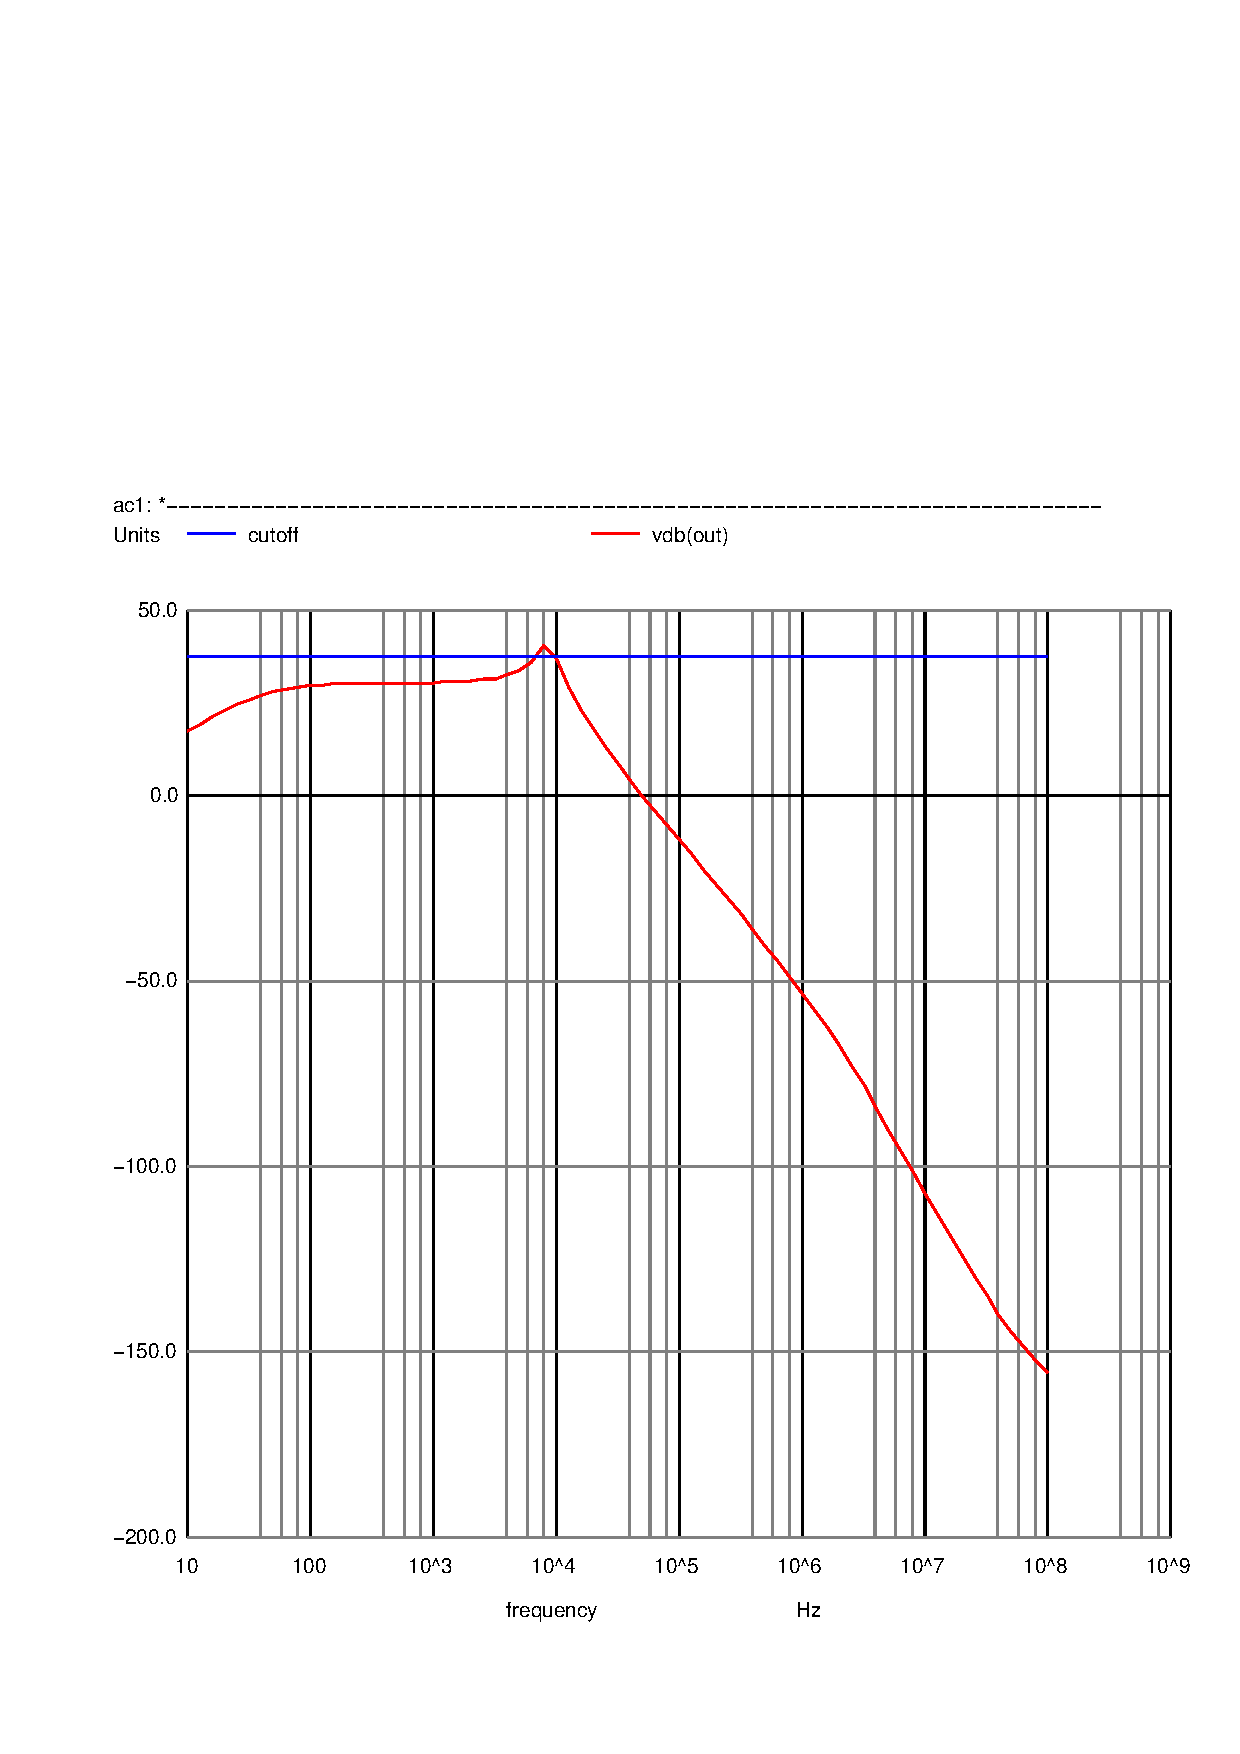
\includegraphics[width=0.3\textwidth, trim={0, 2cm, 0, 8cm}, clip]{vout_mag.pdf}}
	\subfigure[]{\includegraphics[width=0.4\textwidth, trim={0, 6cm, 0, 6cm}, clip]{gain_mag.pdf}}
	\caption{(a) Ngspice and (b) Octave magnitude plots of the frequency response output}
	\label{fig:mag_comp}
\end{figure}

\begin{figure}[h]
	\centering
	\begin{minipage}[t]{.4\textwidth}
		\centering
		\small
		\begin{tabular}{|c|c|}
		\hline
		\input{out_tab.tex}
		\normalsize
		\end{tabular}
	\end{minipage}
	\medskip
	\begin{minipage}{.4\textwidth}
		\centering
       	\input{results.tex}
	\end{minipage}
	\label{fig:op_comp}
	\caption{Results(a) Ngspice (b) Octave script}
\end{figure}

As we can see, both the results for the simulation and the theoretical analysis are very similar, in order to better see this agreement we can look at the relative error between the results:

\begin{figure}[h]
	\centering
	\begin{tabular}{|c|c|}
		\hline
		Quantity & Relative Error (\%) \\ \hline
		Lower Cutoff Frequency & -2.45321 \\ \hline
		Central Frequency & -7.62450 \\ \hline
		Upper Cutoff Frequency Frequency & -12.52166 \\ \hline
		Input Impedance & -0.496051, 21.38860\\ \hline
		Output Impedance & 0, 0\\ \hline
		Gain & 6.833636 \\ \hline
	\end{tabular}
\end{figure}

These relative errors are small in some cases (Lower cutoff freq, central freq, output impedance and gain), however, there are some differences which we can explain due to the difference between the theoretical model and the real OP-AMP component. 

\subsection{The Theoretical OP-AMP Model}
\hspace{12pt} Finally, we will take a look at the theoretical model used back in section \ref{sec:theory}, it is possible to see that, due to its simplicity, it would be very difficult to accurately represent the effect of the OP-AMP, the main difference we experienced is related to the frequency response: given that the theoretical model only includes 2 resistors and a voltage controled voltage source, it cannot model the frequency effects the real component represents (which contains 2 capacitors), this results in the difference in shape we can see in the bode plots.

\begin{figure}[h]
 	\centering
	\includegraphics[width=.5\textwidth, trim={0 2cm 0 5cm}, clip]{OP_AMP.pdf}
	\vspace{-20pt}
	\caption{OP-AMP amplifier incremental model}
	\label{fig:OP-AMP}
\end{figure}


\end{document}
